\documentclass[a4paper,14pt]{extarticle} 
\usepackage[a4paper,top=1.5cm, bottom=1.5cm, left=2cm, right=1cm]{geometry}
%\usepackage[T2A]{fontenc}
%\usepackage[english, russian]{babel}
\usepackage{graphicx}
\DeclareGraphicsExtensions{.pdf,.png,.jpg}

\usepackage{fontspec}
\setmainfont{Times New Roman}
\setsansfont{FreeSans}
\setmonofont{FreeMono}
\renewcommand{\baselinestretch}{1.5}
\usepackage{polyglossia}
\setdefaultlanguage{russian}
\setotherlanguages{english,russian}
\usepackage{setspace}
\usepackage[many]{tcolorbox}
\usepackage{listings}
\usepackage{xcolor}

\definecolor{codegreen}{rgb}{0,0.6,0}
\definecolor{codegray}{rgb}{0.5,0.5,0.5}
\definecolor{codepurple}{rgb}{0.58,0,0.82}
\definecolor{backcolour}{rgb}{0.95,0.95,0.92}

\lstdefinestyle{mystyle}{
    backgroundcolor=\color{backcolour},   
    keywordstyle=\color{magenta},
    numberstyle=\tiny\color{codegray},
    stringstyle=\color{codepurple},
    basicstyle=\ttfamily\footnotesize,
    breakatwhitespace=false,         
    breaklines=true,                 
    captionpos=b,                    
    keepspaces=true,                 
    numbers=left,                    
    numbersep=5pt,                  
    showspaces=false,                
    showstringspaces=false,
    showtabs=false,                  
    tabsize=2
}

\lstset{style=mystyle}
\setlength{\parindent}{5ex}


\begin{document}
    \begin{center}
        \thispagestyle{empty}
        \begin{singlespace}
        ФЕДЕРАЛЬНОЕ АГЕНТСТВО СВЯЗИ

        ФЕДЕРАЛЬНОЕ ГОСУДАРСТВЕННОЕ БЮДЖЕТНОЕ ОБРАЗОВАТЕЛЬНОЕ

        УЧРЕЖДЕНИЕ ВЫСШЕГО ОБРАЗОВАНИЯ

        «САНКТ-ПЕТЕРБУРГСКИЙ ГОСУДАРСТВЕННЫЙ УНИВЕРСИТЕТ ТЕЛЕКОММУНИКАЦИЙ ИМ. ПРОФ. М.А. БОНЧ-БРУЕВИЧА»

        (СПбГУТ)
        \end{singlespace}
        \vspace{-1ex}
        \rule{\textwidth}{0.4pt}
        \vspace{-5ex}

        Факультет \underline{Инфокоммуникационных сетей и систем}

        Кафедра \underline{Защищенных систем связи}
        \vspace{10ex}

        \textbf{Лаборатоoрная работа №3}\\
        Назначение политик безопасности в Центре обеспечения
        безопасности Клиентской консоли Falcongaze SecureTower
        

    \end{center}
    \vspace{4ex}
    \begin{flushright}
    \parbox{10 cm}{
    \begin{flushleft}
        Выполнили студенты группы ИКТЗ-83:

        \underline{Громов А.А., Миколаени М.С., Мазеин Д.С.} \hfill \rule[-0.85ex]{0.1\textwidth}{0.6pt}

        \footnotesize \textit{ (Ф.И.О., № группы) \hfill (подпись)} \normalsize

        Проверил:

        \underline{Казанцев А.А.} \hfill \rule[-0.85ex]{0.1\textwidth}{0.6pt}

        (\footnotesize \textit{уч. степень, уч. звание, Ф.И.О.) \hfill (подпись)} \normalsize

    \end{flushleft}
    }
    \end{flushright}
    \begin{center}
        \vfill
        Санкт-Петербург

        2021

    \end{center}
    \newpage

    \textbf{Цель лабораторной работы:}

    Научиться управлять работой Центра обеспечения безопасности Клиентской консоли Falcongaze
    SecureTower, получить опыт создания правил безопасности различных типов, освоить работу с 
    уведомлениями об инцидентах безопасности.

    \textbf{Пункт 2.9 - Добавление правил}
    \begin{center}
        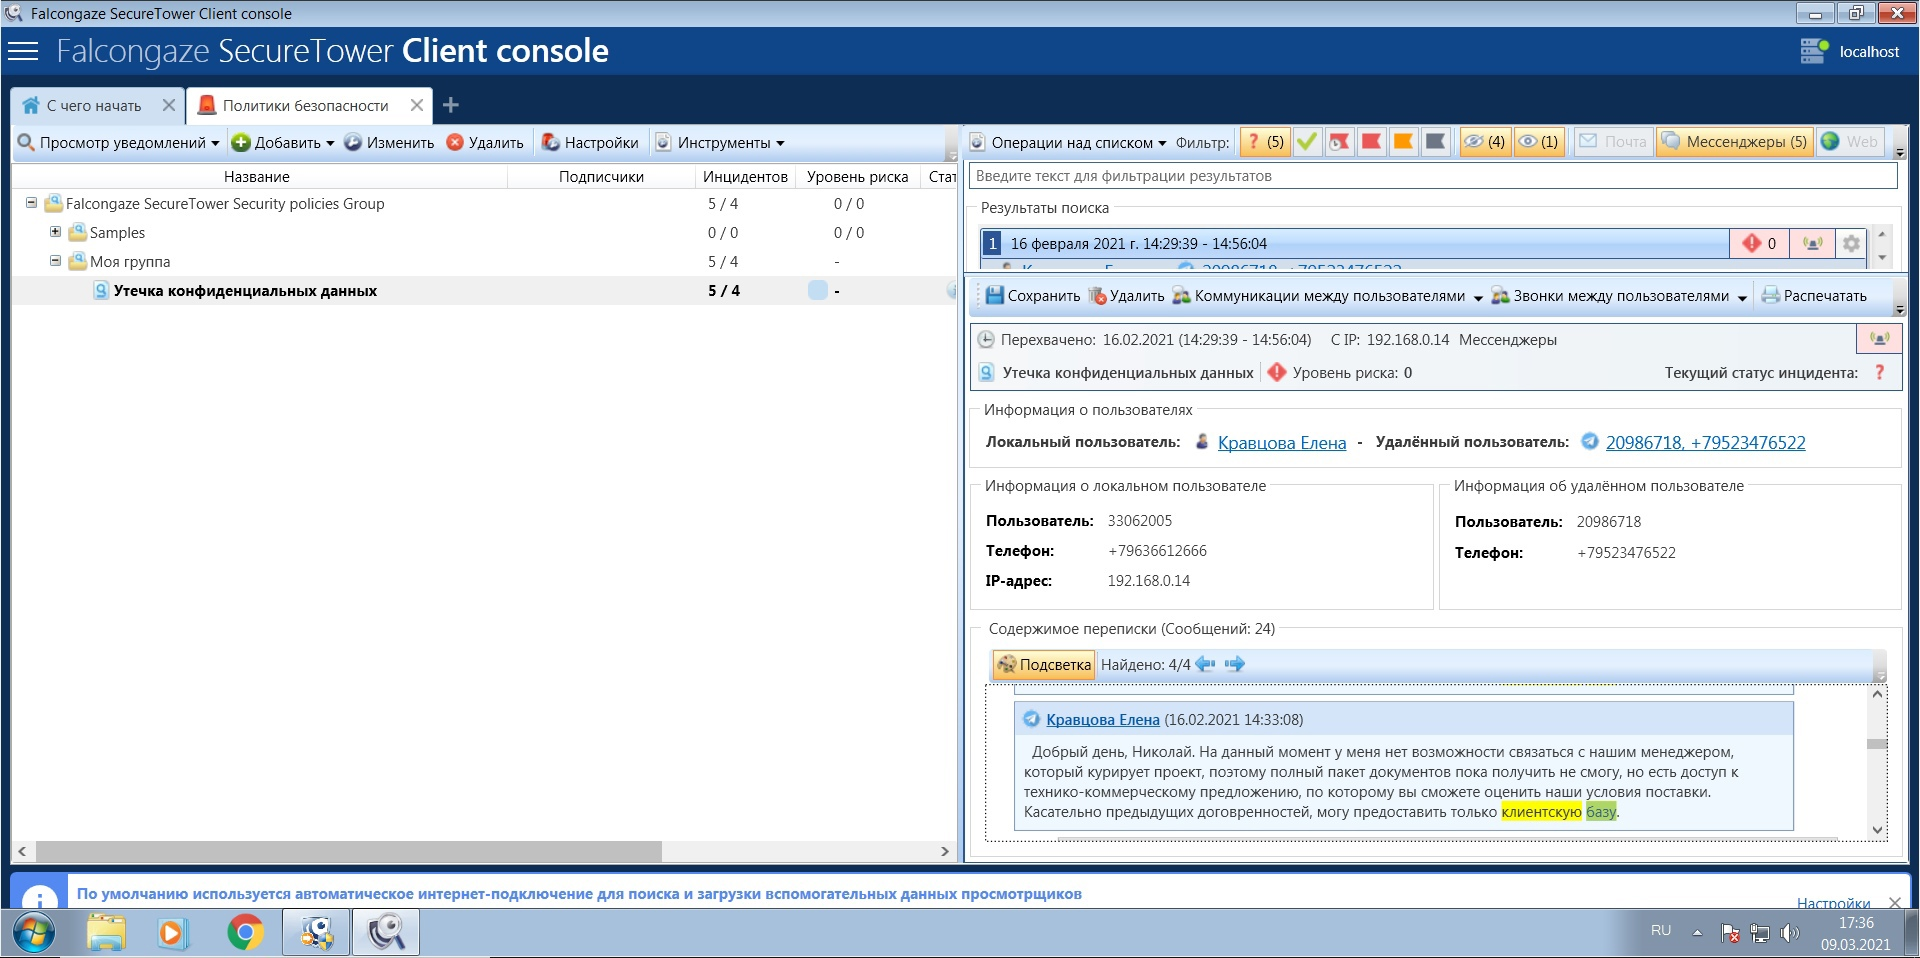
\includegraphics[scale=0.25]{pics/2.9.jpg}

        Правило отображается в папке Мои правила.
    \end{center}

    \textbf{Пункт 3.4.5 - Создание словаря}
    \begin{center}
        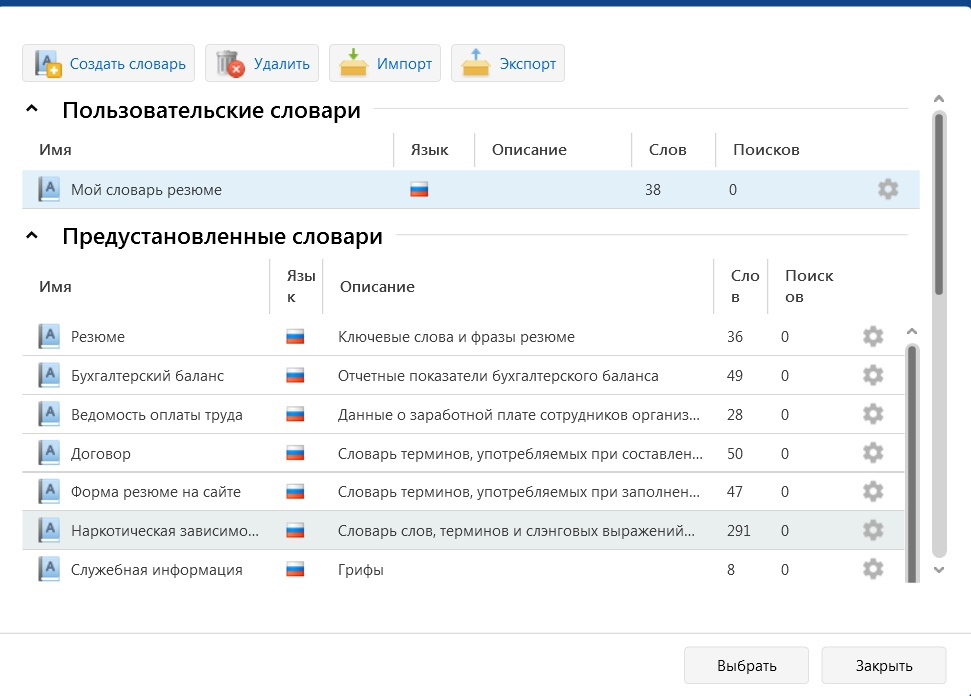
\includegraphics[scale=0.4]{pics/3.4.5.jpg}
        
        Имя словаря отображается в поле списка Словарь.
    \end{center}

    \textbf{Пункт 3.9 - Применение правила для вывода результатов}
    \begin{center}
        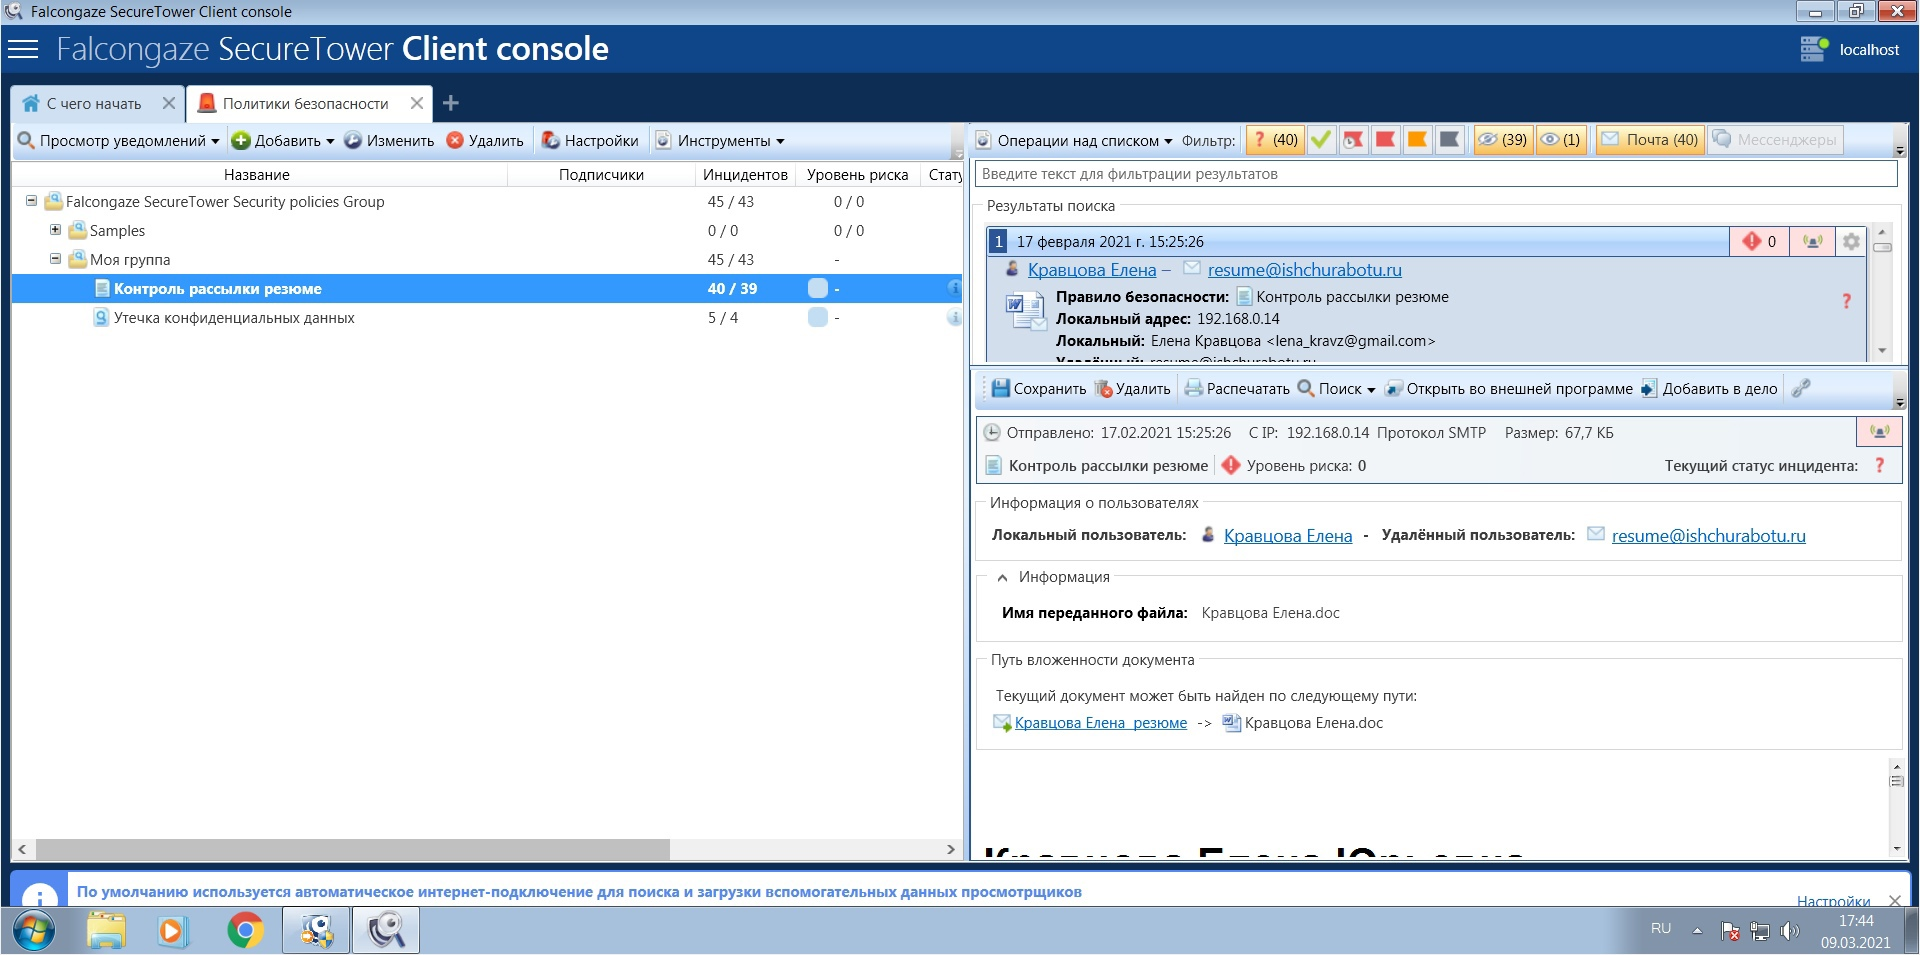
\includegraphics[scale=0.25]{pics/3.9.jpg}

        В результате обработки правила обнаружено 20 инцидентов
        безопасности.
    \end{center}

    \textbf{Пункт 4.6.2 - Применение правила для вывода результатов} 
    \begin{center}
        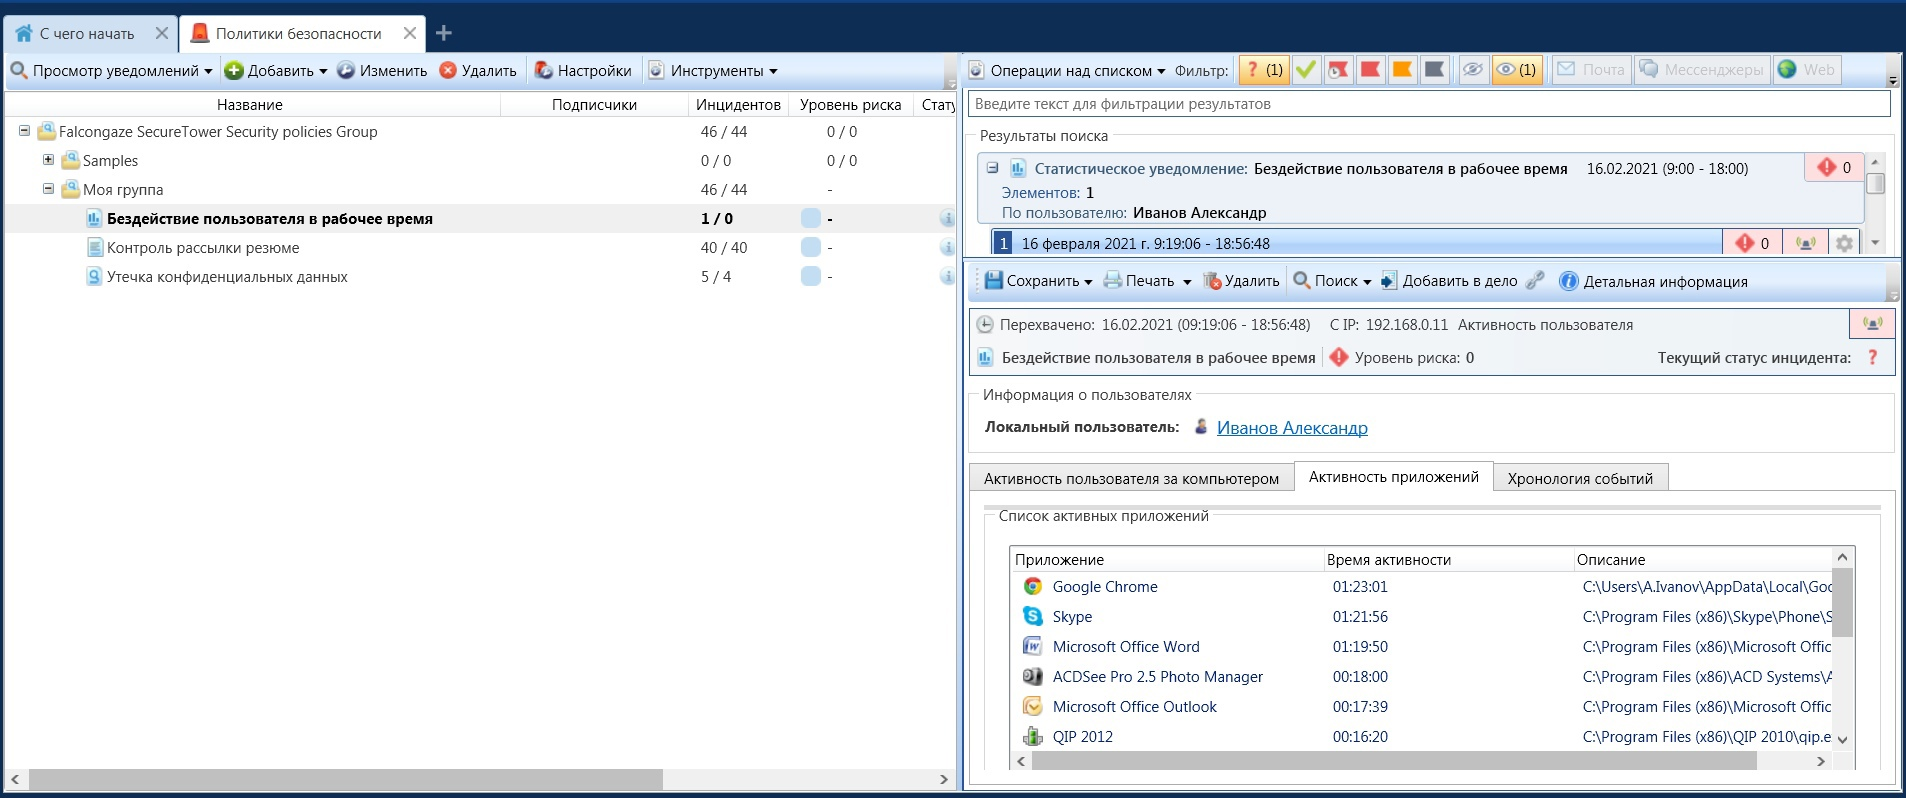
\includegraphics[scale=0.25]{pics/4.6.2.jpg}

        В результате обработки правила обнаружено 1 инцидента безопасности. 
    \end{center}

    \textbf{Пункт 5.2.3 - Добавление банка цифровых отпечатков}
    \begin{center}
        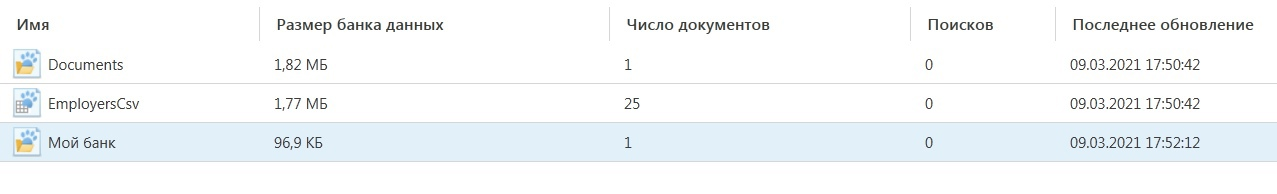
\includegraphics[scale=0.25]{pics/5.2.3.jpg}

        Имя банка отображается в списке цифровых отпечатков.
   \end{center}

    \newpage
    \textbf{Пункт 5.9 - Применение правила для вывода результатов}
    \begin{center}
        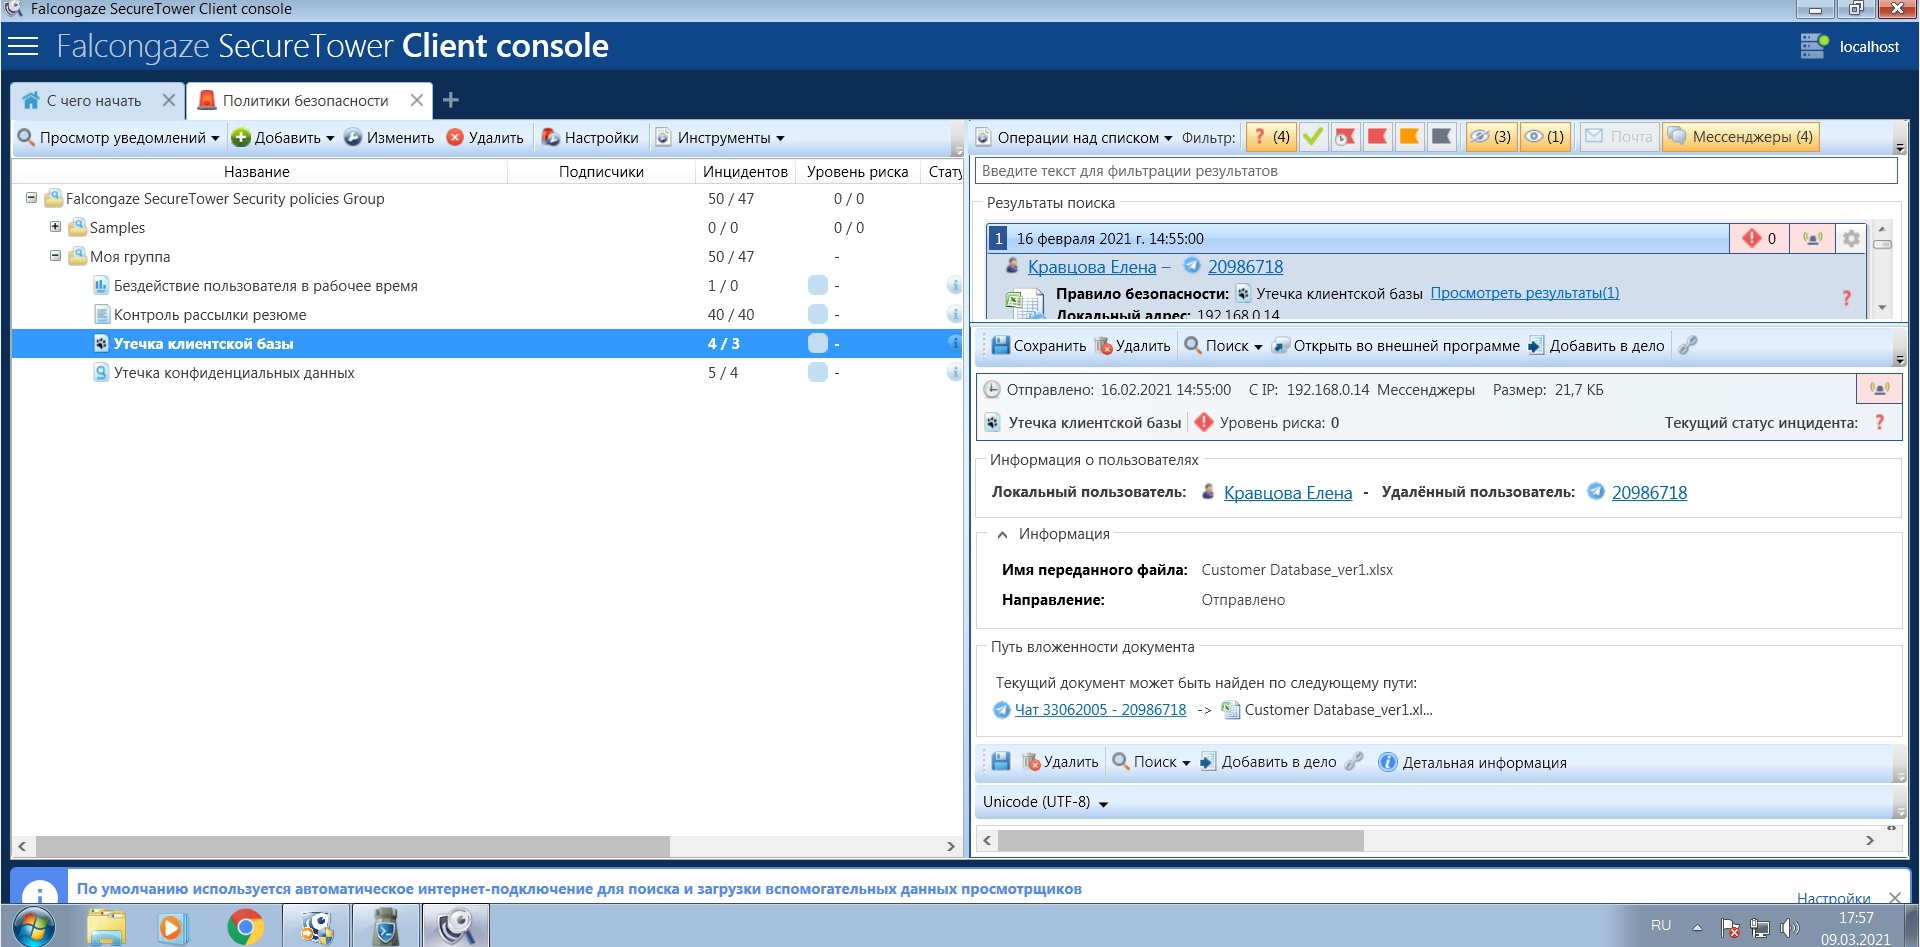
\includegraphics[scale=0.25]{pics/5.9.jpg}

        В результате обработки правила обнаружен 1 инцидент безопасности.
    \end{center}

    \newpage
    \textbf{Выводы:}

    В отличие от лабораторных работ 2.1 и 2.2, нами была произведена автоматизация контроля 
    утечек информации и оповещение об этих инцидентах посредством SMTP. Автоматизация может 
    быть произведена по 4 фильтрам: ключевые слова, словари, цифровые отпечатки, 
    статистические правила.
    
    \textbf{Ответы на контрольные вопросы.}
    \begin{enumerate}
        \item \textbf{ Какие способы используются в системе SecureTower для оповещения о
        сетевых событиях, нарушающих политику безопасности?}

    \qquad Только SMTP-сервер. 
        \item \textbf{ Какие виды правил безопасности доступны в Центре обеспечения
        безопасности?}

    \qquad Обычное, контроль по словарю, статистическое, цифровые отпечатки
        \item \textbf{ Для каких источников данных доступна возможность создания цифровых
        отпечатков?}

    \qquad Для банков данных.
        \item \textbf{ В чем основные отличия контроля по тексту, по словарю от контроля за
        событиями безопасности по цифровым отпечаткам? }

    \qquad Поиск по цифровым отпечаткам ищет документы, по тексту ищет слова, по словарю - тематический поиск.
   \end{enumerate}
    \end{document}